\documentclass[12pt,a4paper,onecolumn]{scrartcl}
\usepackage[utf8]{inputenc}
\usepackage{amsmath}
\usepackage{amsfonts}
\usepackage{amssymb}
\usepackage[ngerman]{babel}
\usepackage[left=2.5cm,right=2.5cm,top=2.5cm,bottom=2.5cm,head=14.5pt]{geometry}
\usepackage{scrlayer-scrpage} % Zur Anpassung der Kopf- und Fußzeilen
\usepackage{graphicx}
\usepackage{float}
\usepackage{lmodern}
\usepackage{mathtools}
\usepackage{graphicx}
\usepackage{subfig}
\usepackage{caption, booktabs}
\usepackage{paralist}
\usepackage[toc,acronym,nonumberlist,translate=babel]{glossaries}
\usepackage{underscore}
\usepackage{float}
\usepackage{wrapfig}
\usepackage{array}
\usepackage{adjustbox}
\usepackage{makecell}
\usepackage{pdfpages}
\usepackage{csquotes}
\usepackage{hyperref}
\usepackage{chngcntr} % Damit Zählungen von Abb und Co innerhalb sections mögl
%\usepackage[scaled]{uarial} % Schriftart
\usepackage{url}

\usepackage[backend=biber,natbib=true,hyperref=true,
			style=draft,maxnames=2,maxbibnames=2, isbn=false]{biblatex}
% STYLE draft SPÄTER NOCH GEGEN authoryear TAUSCHEN!!!!!!
\addbibresource{literatur.bib} %% Einbinden der bib-Datei
\DefineBibliographyStrings{ngerman}{
	andothers = {{et\,al\adddot}},}

\def\theequation{\thesection.\arabic{equation}} % Formeln beginnen mit Abschnittssnummer
\linespread{1.0} % Zeilenabstand
\pagestyle{scrheadings}
\clearpairofpagestyles % Löschen der Platzhalter
\counterwithin{figure}{section} % damit figure je section neu gezählt werden

\newcommand*\mytitle{Arbeitstitel: Eisenhypothese Dust-Event 2009}
\newcommand*\mysubtitle{Bachelorarbeit}
\newcommand*\myauthor{Marco Schulz}
\newcommand*\mydate{05.03.2021}
\newcommand{\cotwo}{CO\textsubscript{2}}

\begin{document}
\begin{titlepage}
\begin{center}
{\LARGE \textsc{\mysubtitle}} \bigskip \\
{\huge \textsf{\mytitle}} \bigskip \\
{\Large \myauthor \ - Matrikelnummer 7345692} \smallskip \\
{\Large Fassung vom \mydate} \bigskip \\
\begin{figure}[H]
\centering

\includegraphics[width=60mm]{bilder/unilogo.png}
\end{figure}
\bigskip
{\Large Institut für Geophysik und Meteorologie}
\bigskip
{\Large \\ Universität zu Köln}
\vspace{4cm}
\\
\end{center}
\noindent Erstgutachter: Prof. Yaping Shao (yshao@meteo.uni-koeln.de)
\bigskip \\
Zweitgutachter: Prof. Joachim Saur (saur@geo.uni-koeln.de)
\end{titlepage}
\setcounter{page}{2}
\ofoot{\pagemark}
\chead{{\small \mytitle}}
\automark{section}
\tableofcontents
\newpage
\begin{abstract}
DIESEN QUATSCH HABE ICH MIT DEM IPAD GESCHRIEBEN
Das kann ich erst am Ende schreiben!
\end{abstract}
\section{Einleitung}
Klima verändert sich. Aktuell Eiszeitalter. Glaziale, Interglaziale abwechselnd. Bekannt (aus Eisbohrkernen), dass geringe \cotwo -Konzentration in Atmosphäre während Glazialen. Deckt sich mit den geringen Temperaturen. Wohin das ganze \cotwo ? Phytoplankton sorgt für $50\%$ des jährlichen \cotwo -Austauschs \citep{Field.1998} und erzeugen etwa 45 gt organischen Kohlenstoff pro Jahr \citep{Falkowski.1998}. Phytoplankton benötigt \cotwo \ zum Wachsen, wodurch dieses zu Biomasse konvertiert wird. Somit bei erhöhten Phytoplankton weniger \cotwo . Warum wächst Phytoplankton dann nicht beständig, bis alles \cotwo\ aufgebraucht? Weitere limitierende Faktoren, da zur Fotosynthese weitere Nährstoffe benötigt werden. Nitrat und Phosphate als Nährstoffe, auch von Tiefsee. \citet{Martin.1988} zeigen, dass Eisen limitierender Faktor. Eiseneintrag hauptsächlich aus Staub. Wenige Staubquellen in Südhemisphäre bzw. südl. Ozean (vgl. China/Sahara). Dadurch Eisenmangel, hingegen reich an Nitraten und Phosphaten aufgrund Upwelling (aufgrund Ekmantransport der zyklonalen Zirkumpolarströmung). Falls dann doch größere Eisendeposition, Phytoplankton-Blüten. Dies als mögliche Erklärung für geringe \cotwo - Konzentrationen während Glazialen (Modelle zeigen, dass dies ungefähr die Hälfte des \cotwo \ Rückgangs erklären könnte. Etwa 16 gt Kohlenstoff werden aktuell pro Jahr durch die biologische Pumpe im Ozean archiviert \citep{Falkowski.1998}. Wenn diese Hypothese angenommen, dann bei größeren Staub-Events (kleine Zeitskala) vermehrtes Phytoplankton Wachstum wahrscheinlich. Ein großes Event 2009 in Australien. Dieses soll in dieser Arbeit genauer untersucht werden. Abgleich Staub- bzw. Eisendeposition mit Entwicklung Phytoplankton (bzw. Chlorophyll-$\alpha$). Dazu benutze Kölner WRF-Staub-Weiterentwicklung. Vergleich mit Satellitenbildern. Nutze verschiedene Verfahren der Statistik. Berücksichtige Ozeanzirkulation und Wind. Falls Zusammenhang gezeigt werden kann dann Hypothese wahrscheinlich. Wäre weiteres Indiz für Eisenhypothese. Wurde schonmal gemacht \citep{Gabric.2016}. Prüfung des Kölner Modells. Zusammenhang $\Rightarrow$ ggf. ebenfalls Hinweis dass Modell gut.
\section{Gabric.2016}

\begin{itemize}
\item Tasman Sea $25^\circ$ S bis $40^\circ$ S Untersuchungsareal
\item data: Chl + aeorosol optical depth (AOD)
\begin{itemize}
\item chl data: dialy + 8 day MODIS-AQUA
\item AOD data: 550 nm, 4km resolution 
\end{itemize}
\item divided into $5^\circ$ lattitude band
\item DVR kumulativ
\item Hovmoller Plots (x: zeit, y: latidude, longitude)
\item cloud processing / wet deposition wichtig
\item Response hauptsächlich südlich der tasmanischen Front ($\approx 32^\circ$ S) 
\item Staubdeposition weiter im Norden

\end{itemize}

\section{Theorie}
\subsection{Kohlendioxid und Klima}
\subsection{Wachstum von Phytoplankton}
Kurz: Welcher Prozess passiert genau bei Nährstoffe $\Rightarrow$ Phytoplankton / Fotosynthese \\\\
Phytoplankton sind Einzeller.
Wachstumsbeeinflussende Faktoren sind \citep{Falkowski.1998}):
\begin{enumerate}
\item mixed-layer depth
\item nutrient fluxes
\begin{enumerate}
\item Phospor \citep{REDFIELD.1960}
\end{enumerate}
\item food-web structure
\end{enumerate}
\citet{Boyce.2010} folgern, dass der Reichtum an Phytoplankton insgesamt seit Beginn der Messungen (1899) aufgrund der Erwärmung der Ozeane abgenommen hat. Es wird geschätzt, dass das globale Median jährlich um etwa 1\% abnimmt. Da die Klimamodelle steigende (Meeres-)Temperaturen prognostizieren ist es wahrscheinlich und problematisch, dass die Menge an Phytoplankton, der Basis aller Nahrungsketten im Ozean, zukünftig noch weiter abnimmt \citep{Siegel.2010}. Klimaänderungen werden direkt (andere Ozeanchemie) und indirekt (Änderungen in der Ozeanzirkulation) die Verteilung des Phytoplanktons verändern \citep{Falkowski.1998}. Mithilfe Temperatur des Oberflächenwassers, einfallender Sonnenstrahlung, mixed-layer-depth, Up- und Downwellingzonen kann aus CHL-a Konzentration die NPP abgeleitet werden \citep{Falkowski.1998}. Für Kieselalgen ist Zufuhr von Kieselsäure essenziell; diese tritt fast ausschließlich südlich der Südpolarfront auf \citep{Falkowski.1998}.
\\\\
elemental composition of phytoplankton (106C/16N/1P) \citep{Falkowski.1998}

\subsection{Eisenhypothese}
Andere Nährstoffe für Phytoplankton können durch aufsteigendes Tiefenwasser bereitgestellt werden. Eisen und Mangan werden hingegen hauptsächlich durch äolischen Staub eingebracht. Verweildauer von etwa 6 Monaten in oberflächennahem Wasser bis ca. 150m Tiefe \citep{Hayes.2015}. Nitrogenase (Enzymkomplex) kann N$_2$ reduzieren und Stickstoff somit biologisch verfügbar machen. Nitrogenase selbst benötigt (bzw. besteht aus) Eisen. Meistens Trichdesmiumspp., das N$_2$ bindet \citep{Falkowski.1998}.
\\\\ Insbesondere im südlichen Ozean kann auch Mangan limitierender Faktor sein \citep{Browning.2021}. Untersuchungen von Eisbohrkernen zeigen, dass Eisenzufuhr durch äolischen Staub in glazialen Perioden um eine Größenordnung größer war als in Interglazialen \citep{Falkowski.1998}.
\begin{figure}[ht]
\centering
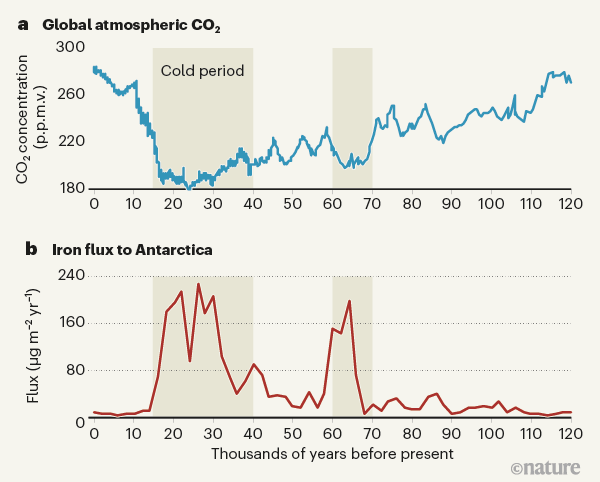
\includegraphics[width=0.7\textwidth]{bilder/Stoll2020/antarctic-iron-global-co2.png}
\caption{Antikorrelation von \textbf{a} globaler \cotwo \ Konzentration und \textbf{b} Eisendeposition in der Antarktis \citep{Stoll.2020}}
\end{figure}
\subsubsection{Düngung funktioniert nicht}
verschiedene Ursachen. Verweilzeit in Oberflächenwasser \citep{Hayes.2015}. Aufnahmefähigkeit / Rezeptivität ist saisonal variabel \citep{Gabric.2016}, Sekundärquelle. In nährstoffarmen Gewässern haben extrem kleine Phytoplankton-Organisamen bei der Verarbeitung von Nährstoffen (Exkrementen der Verbraucher) einen Wettbewerbsvorteil, da großes Oberflächen zu Volumen- Verhältnis \citep{Falkowski.1998}.Wenn hingegen \textit{neue} Nährstoffe bspw. durch Upwelling nach oben gelangen, hat größeres Phytoplankton, insbesondere Kieselalgen einen Wettbewerbsvorteil (aufgrund Vakuole, schnellere Aufahme). Das Plankton, das sich wiederum von diesen ernährt, ist typischerweise größer, benötigt für Entwicklung (Larvenstadium) mehr Zeit; dadurch im gegensatz zu obigen Arealen Blooms möglich und stärkere biologische Pumpe. \citep{Falkowski.1998}. Zeitreihen für Messungen der Ozeanbiologie sind im Vergleich zu Land sehr kurz, wodurch Schätzen auch unzuverlässiger sein können \citep{Falkowski.1998}. Häufigste Beschränkung ist durch Verfügbarkeit von gebundenem anorganischem Stickstoff \citep{Falkowski.1998}.
\subsubsection{Biologische Pumpe}
Niedriger Sauerstoffgehalt in der Tiefsee weist auf starke biologische Pumpe hin (dortige durch mehr absinkendes Plankton angereicherte Organismen verbrauchen mehr Sauerstoff?). Im aktuellen Ozean beträgt der (Sink)Fluss ca. 16 Pg Kohlenstoff pro Jahr \citep{Falkowski.1998}. In Küstengebieten (Upwelling) sehr deutlich $\Rightarrow$ Fischerei profitiert. Hoher Sauerstoffgehalt führt zu oxidiertem Eisen; oxidiertes Eisen ist nicht löslich und sinkt $\Rightarrow$ geringer Eisengehalt \citep{Falkowski.1998}


\subsection{Staubkreislauf}
wichtige Verbindung zu Energie- und Kohlenstoffkreislauf \citep{Shao.2011}
\subsubsection{Staubquellen in Australien}
größte Teil Zentralaustralien \citep{Shao.2011} siehe auch Lake Eyre basin
\subsubsection{Eisen in Staub}
Nicht jede Form von Eisen kann als Dünger dienen. Muss entsprechend gelöstes (?) Eisen sein. Transportprozesse und Wolkenbildungen können die Transformation zu diesem tauglichen Eisen fördern \citep{Shao.2011}. Die Planktonart Trichodesmium kann die Rate des Eisenauflösens von Oxiden und Staub beschleunigen (im Gegensatz zu anderem Phytoplankton) \citep{Gabric.2016}
\subsubsection{Emissions- und Depositionsmodelle}
ggf. lieber in Kapitel Methoden
\subsection{Wind und Oberflächenströmungen}
Verkleinerung der Tiefe der Oceanic Mixed Layer von September auf Oktober \citep{Tilburg.2002} (abchecken, dass der Bloom nicht daher kommt!). Einteilung in \textit{nördlich der Tasmanischen Front} und \textit{südlich der tasmanischen Front}? Phytoplanktonproduktion hängt von Up- und downwelling-Prozessen durch mesoskalige Wirbel ab \citep{Tilburg.2002} $\Rightarrow$ Vorticity der Ozeanströmungen berechnen?Besser sea surface height (SSH) Anonmalien angucken. Was, wenn Blüte bei \citet{Gabric.2016} aufgrund von tieferen mixed-layer aufgrund des Sturms? $\Rightarrow$ Winddaten vergleichen. 
\section{Beschreibung des Staubsturms in September 2009}
stärkstes (in Bezug auf Sichtweitenreduzierung) Staubevent über Sydney seit es verlässliche Aufzeichnungen gibt (1940, \citet{Leys.2011}). Staubstürme üblich im ariden Inland. Vorangegangen sind Monate und Jahre mit im Vergleich zum Durchschnitt höheren Temperaturen und unterdurchschnittlichem Niederschlag; dadurch schwache Vegetation und trockene Erdböden \citep{Leys.2011}.
\section{Wetter}

\section{Staubtransport}
Staubquellen gemäß \citep{Leys.2011} 
\begin{enumerate}
\item lower Lake Eyre Basin
\item grazing lands of north western NSW
\item mining areas around Cobar und Broken Hill
\item Channel Country of western Queensland
\end{enumerate}



\section{Methoden}
hole Zeitreihe Chlorophyll alpha Entwicklung von September bis Oktober (bzw. falls saisonale Veränderung, den Zeitraum, welcher der Kurve Dust-Event-Zeitraums entspricht) gemittelt über bspw. 10 Jahre. Berechne daraus Anomalie 2009 und vergleiche diese mit Staubdeposition.
\subsection{iron residence time modell}
\subsection{phytoplankton response time modell}
turn-over time ist von Größenordnung einer Woche oder weniger \citep{Falkowski.1998}: abgeleitet durch: 45 bis 50 Pg Kohlenstoff produzieren Phytoplankton pro Jahr, aktuell im Ozean sind aber immer nur ca. 1 Pg, das heißt dass das jeweils aktuelle Phytoplankton immer nach ca. einer Woche \textit{umgesetzt} wurde.

\subsection{WRF Modell}
nur kurze Vorstellung, da grundsätzlich nur der Output verwendet werden soll. Vergleich mit von \cite{Gabric.2016} genutzem Modell CEMSYS
\subsection{Phytoplankton}
Climate Data Store \nocite{*}
\\\\
Messungen des Chlorphyll-$\alpha$ geben Rückschluss auf Phytoplankton \citep{RYTHER.1957}(muss ich noch lesen)

\subsection{EOF?}
\subsection{Riegers Principal Components?}

\section{Auswertung und Diskussion}
\section{Zusammenfassung und Ausblick}
\newpage
\printbibliography
\newpage
\appendix
\section{Anhang}
\addcontentsline{toc}{section}{Abbildungsverzeichnis}
\listoffigures
\addcontentsline{toc}{section}{Tabellenverzeichnis}
\listoftables
\section{Danksagung}
\end{document}
